\graphicspath{{./images/chap5/}}
% Sloop-mturk: Crowdsourced relevance feedback on mturk
% Methodology
% * Design and Architecture
% * Population of interest and sampling subject used in the study
% * Instrument and what it measures (metrics)
% * qualifications of informants if used in the study
% * Validation
% * Data gathering procedure (experiments)
\chapter{Crowdsourced Relevance Feedback}
\label{chap:sloop_mturk}
% Sloop-mturk: Crowdsourced relevance feedback on mturk
\section{Sloop MTurk}

As described in Chapter~\ref{chap:relevance_feedback}, multiple rounds of
relevance feedback accretes precision and recall. This
chapter presents the architecture of \emph{Sloop MTurk}, the crowdsourced
relevance feedback engine for Sloop.

\begin{figure}[htb]
  \centering
  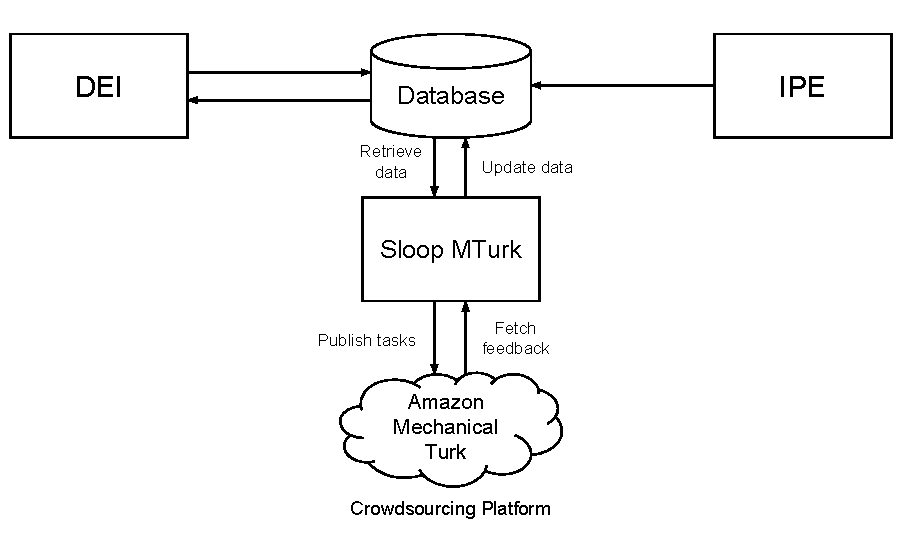
\includegraphics[width=0.8\textwidth]{sloop/turk_system}
  \caption{Sloop Architecture with Sloop MTurk integration}
  \label{fig:turk_overview} %chktex 24
\end{figure}

Sloop MTurk communicates with the crowdsourcing platform in order to obtain
human feedback on the original rankings. Our focus is on

\subsection{Architecture}

There are four major functions used within the relevance feedback
workflow: Retrieve, Publish, Fetch, and Update.

\subsubsection{Retrieve}

In the first stage of the relevance feedback workflow, Sloop MTurk retrieves a
number of known and unknown image pairs from the database in the ratio
described in Section~\ref{subsub:validation}. The metadata about the retrieved
pairs, such as the answers to the known pairs, individual identification
numbers, and source address, is stored in a lightweight SQLite database.

Sloop MTurk never publishes a duplicated \emph{unknown} pair onto MTurk. It
actively checks with the local database before any retrieval whether an unknown pair
has ever been published before. Users can set the sampling policy of Sloop MTurk in
the configuration file. The default is to use the normal sampling from the
median whose performance has been shown in
Chapter~\ref{chap:relevance_feedback}.

Sloop MTurk only fetches from the Sloop database the images necessary for the
tasks to be published.  Upon retrieval, Sloop MTurk caches the image data
locally on the filesystem behind NGINX\@. Caching image data reduces data transfer
overhead because fetching large responses (like images) over the network is
both slow and expensive.

\subsubsection{Publish}

Sloop MTurk publishes the tasks to MTurk immediately after all the
information is fetched. The tasks published are available on Amazon Mechanical
Turk under the title: `Image Matching --- Animals' posted by user `sloop'.
% TODO Tell user that they need AWS access ID and secret key to
% programmatically communicate with MTurk

\subsubsection{Fetch}

Users can fetch results once the published tasks have been completed. This can
be run as a cron job.  For each completed task with correct answers to all
known pairs, Sloop MTurk accepts and retrieves the results, allowing the worker
to be paid.  For any tasks with incorrect answers to known pairs, Sloop MTurk
rejects the results, with no payment given.

Sloop MTurk logs the answers to the unknown pairs from the accepted assignments
in the local SQLite database. Results are never deleted automatically.

\subsubsection{Update}

The update command pushes the answers logged in the local SQLite database back
to the original Sloop database so that the data is ready for another round of
relevance feedback. The remote database server then categorizes the captures
with the data pushed and the existing data, and then performs its cohort
merging logic~\cite{sloopdocs}.

The update command is separated from fetch for ease of debugging. In
practice, we would like to update the upstream database as frequently as
possible as we have seen in the Experiments section,
Chapter~\ref{chap:relevance_feedback}.

\subsection{Platform Selection}

Workers and requesters interact via a crowdsourcing platform. All our tasks
are published on Amazon Mechanical Turk (MTurk), which is one of the most
popular crowdsourcing platforms.

\subsection{Human Intelligence Task (HIT)}

Tasks published on MTurk are called Human Intelligence Tasks (HITs). The terms
`HIT' and `tasks' will be used interchangeably throughout this report.

Requesters publish the tasks that they need completed to Amazon Mechanical
Turk's marketplace with a set payment to reward workers who finish the tasks.

\subsubsection{Task Design}

A wide variety of tasks can be crowdsourced. There are two possible designs we
have considered:
\begin{enumerate}
	\item Rankings and weights \\
    Each worker may be asked to provide a full ranking or relative weights
    for a given pool of candidates. Although knowing the correct rankings is
    valuable to ranked retrieval results,
    ultimately, we would like to determine a sharp cutoff between matching
    images and non-matching images so that each individual can be exclusively
    identified. Ranks alone do not provide such a cutoff. Even if we knew all the
    correct rankings, we would not be able to decide whether two animals are
    the same individual. Thus, rankings and weights is not a viable
    solution.
	\item Multiple-choice questions \\
    A question can include multiple options. For instance, asking which of the images
    in the choices contain an animal that matches the given individual
    animal. However, this approach only tells us which of the pictures among
    all the choices best matches a given image, which is an inefficient
    approach to ranking images. Alternatively, we can ask workers to provide
    all the matches among all the options. In this case, there can be none or
    more than one answer. However, using this method, we only gain the
    information of one individual from $n$ comparisons, where $n$ is the number
    of choices for each question.

    We can model our task as a binary question of whether a pair of images from
    the same view contain the same individual animal (Is a match?).
    Eventually, all the image pairs will be labelled as either a match or a
    non-match, and we will be able to construct a mapping that allows us to
    exclusively identify all the individual animals in the pictures.
\end{enumerate}

\subsubsection{Validation}
\label{subsub:validation}

For each task, since the quality of the submitted work is not directly
observable, we add three other \emph{gold standard} questions, for which the
correct answers are known \emph{a priori}. Among the three questions, one is a known
pair of images containing the same individual, another is a known pair of
images containing different individuals, and the other is a random known pair.
These \emph{gold standard} questions work as qualifying tests for eligible
workers. Additionally, they also accelerate the workers' learning process and
skill level.

To further ensure the correctness of the answers submitted by the workers, we
publish the same assignment to three workers, and determine the correct answer
by consensus. We only allow workers with a task acceptance rate higher than
0.8, to prevent spam. If the majority agrees on some answer, it may be safe to
assume that it is correct. Obviously, the more number of workers we assign to a
given task, the less chance there is of getting an incorrect answer. However,
the budget and the time it takes to complete all the assignments increases
linearly as we increase the number the workers, while the
correctness only increases logarithmically. Therefore, we decided to publish
exactly three assignments, which is the minimum number required to reach a consensus
for each task.

\subsection{Cost Model}

Sloop MTurk uses the evaluation metrics mentioned in
Chapter~\ref{chap:relevance_feedback} to measure the performance of the system.

\subsubsection{Correctness}

To analyze the correctness, we still use the Mean Average Precision.  MAP has
been shown to have especially good discrimination and stability for evaluating
information retrieval
systems~\cite{manning2008introduction}.

\subsubsection{Expense}

Upon completion of a task, each worker receives the posted price for that
task. The more tasks published, the higher the total payment we have to make.
